%        File: 03140299.tex
%     Created: Fri Jan 02 03:00 PM 2015 J
% Last Change: Fri Jan 02 03:00 PM 2015 J
%
\documentclass[10pt,a4paper,twocolumn]{jarticle}

%%%%%%%%%%%%%%%%%%%%%
% to input Japanese %
%%%%%%%%%%%%%%%%%%%%%
\usepackage[japanese]{babel}

%%%%%%%%%%%%%%%%%%%%%
% to insert itembox %
%%%%%%%%%%%%%%%%%%%%%
\usepackage{ascmac}

%%%%%%%%%%%%%%%%%%%%%%%%%%
% to be standard a4paper %
%%%%%%%%%%%%%%%%%%%%%%%%%%
\usepackage{geometry}
\geometry{
  a4paper,
  total={210mm,297mm},
  left=20mm,
  right=20mm,
  top=20mm,
  bottom=40mm,
}

%%%%%%%%%%%%%%%%%%%%%
% to insert figures %
%%%%%%%%%%%%%%%%%%%%%
\usepackage[dvipdfmx]{graphicx}

%%%%%%%%%%%%%%%%%%%%%%%%%%
% to insert source codes %
%%%%%%%%%%%%%%%%%%%%%%%%%%
% \usepackage{listings, jlisting}
% \renewcommand{\lstlistingname}{list}
% \lstset{language=C,
%   basicstyle=\ttfamily\scriptsize,
%   commentstyle=\textit,
%   classoffset=1,
%   keywordstyle=\bfseries,
%   frame=tRBl,
%   framesep=5pt,
%   showstringspaces=false,
%   numbers=left,
%   stepnumber=1,
%   numberstyle=\tiny,
%   tabsize=2
% }

%%%%%%%%%%%%%%%%%%
% title & author %
%%%%%%%%%%%%%%%%%%
\title{ロボットインテリジェンス レポート課題A \\
      「ニューラルネット学習シミュレーション」}
\author{03-140299 東京大学機械情報工学科3年 和田健太郎}

%%%%%%%%%%%%%%%%%%
% begin document %
%%%%%%%%%%%%%%%%%%
\begin{document}
\maketitle

%%%%%%%%%%%%%%%%%%%%%%%%%%%%%%%%%%%%%%%%%%%%%%%%%%%%%%%%
\section{はじめに}
レポート課題として課題Aを選択し, 3層フィードフォワード型の
ニューラルネットとバックプロパゲーション学習をシミュレーション
するプログラムを作成し, 識別実験を行った. 
実験に利用したデータ群は
The MNIST database of handwritten digits
であり, このデータは過去に様々な分類器において
識別能力を図るために利用されている. \cite{mnist}
図\ref{fig:plot-mnist}に実際に利用した学習データの一部を示す. 

\begin{figure}[htbp]
  \centering
  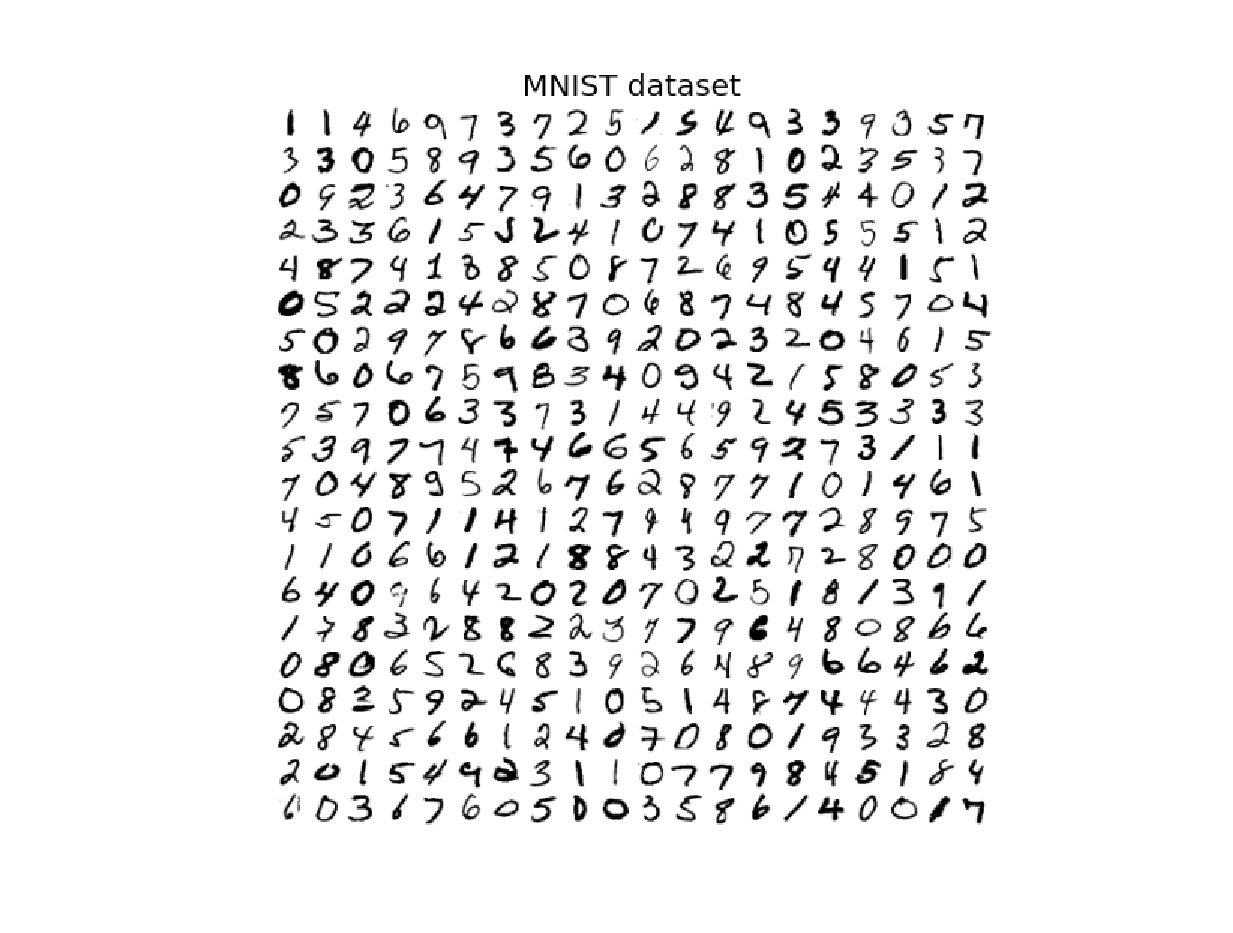
\includegraphics[width=0.45\textwidth]{assets/img/tiled_mnist_nl0.0.eps}
  \caption{MNISTの画像データ}
  \label{fig:plot-mnist}
\end{figure}

また, ノイズを加えた場合の性能変化, ノイズ耐性, 
中間ニューロンの役割, オートエンコーダを利用した画像特徴抽出による
識別性能変化について考察した. 
%%%%%%%%%%%%%%%%%%%%%%%%%%%%%%%%%%%%%%%%%%%%%%%%%%%%%%%%

%%%%%%%%%%%%%%%%%%%%%%%%%%%%%%%%%%%%%%%%%%%%%%%%%%%%%%%%
\section{ニューラルネット学習シミュレーション}
実験に利用したMNISTは, 28 × 28ピクセルのグレースケール手書き数字
画像の70000件のデータセットである. 
データセットを3分割し3分の2を学習データ, 3分の1をテストデータとし, 
以下の様なパラメータに関してモデルの性能を交差検定によって調べた. 

なお, パラメータの検証は以下の順番で行い, 一部を覗いてそれぞれ最良であったものを
次の検証で利用することで, 性能の向上を目指した. 
最初のパラメータ値は, 学習率0.2, 慣性項の係数0, 
隠れ層の数入力の0.1倍, 学習の際のノイズ0とした. 

\begin{itemize}
  \item 学習の際の繰り返し数
  \item 学習率
  \item 慣性項の係数
  \item 隠れ層の数
  \item 学習の際のノイズ率
\end{itemize}

図\ref{fig:epoch-test}が学習の際の繰り返し数を変化させ,
各試行での性能を調べたものである. 
この結果から, 性能は繰り返し回数に従って良くなるということがわかる. 
今回の実験では結果として現れなかったが,
繰り返し回数をさらに増やしていくと, 
性能の向上が打ち止めになり, 過学習によって逆に性能が下がるということが
予想される. 
\begin{figure}[htbp]
  \centering
  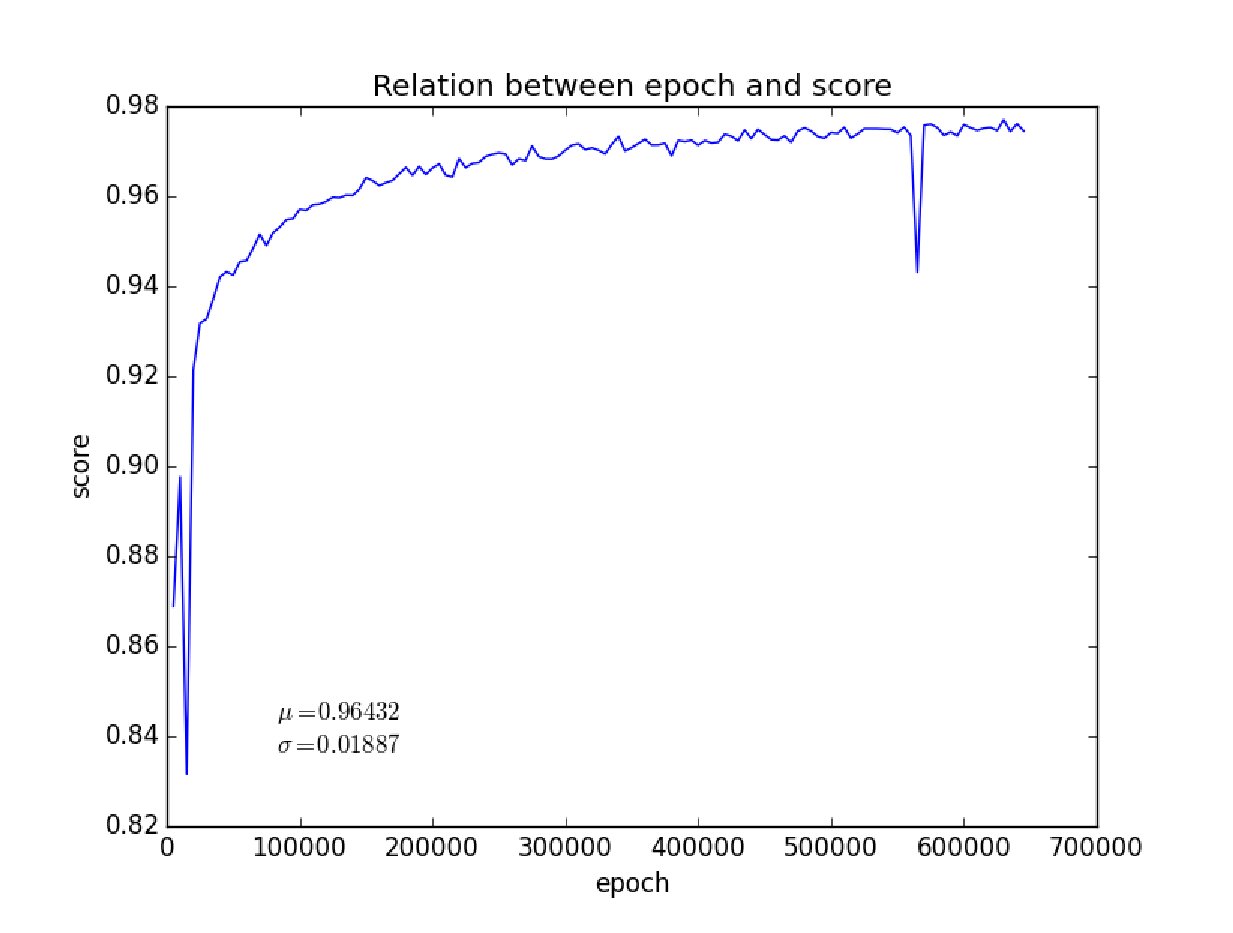
\includegraphics[width=0.45\textwidth]{assets/img/epoch_test_mnist.eps}
  \caption{学習の際の繰り返し数と性能の関係}
  \label{fig:epoch-test}
\end{figure}

図\ref{fig:learning-rate-test}が学習率を0.02から0.4まで変化させ, 
性能の変化を調べたものである. 
この結果から, 0.25以降は変化が小さいことがわかる. 
最良の性能を出したのは, 学習率が0.3の時であった. 
また, 0.2のときのように性能が大きく下がるパラメータ値もあるため, 
パラメータを変化させて性能を検証することの必要性がわかる. 
\begin{figure}[htbp]
  \centering
  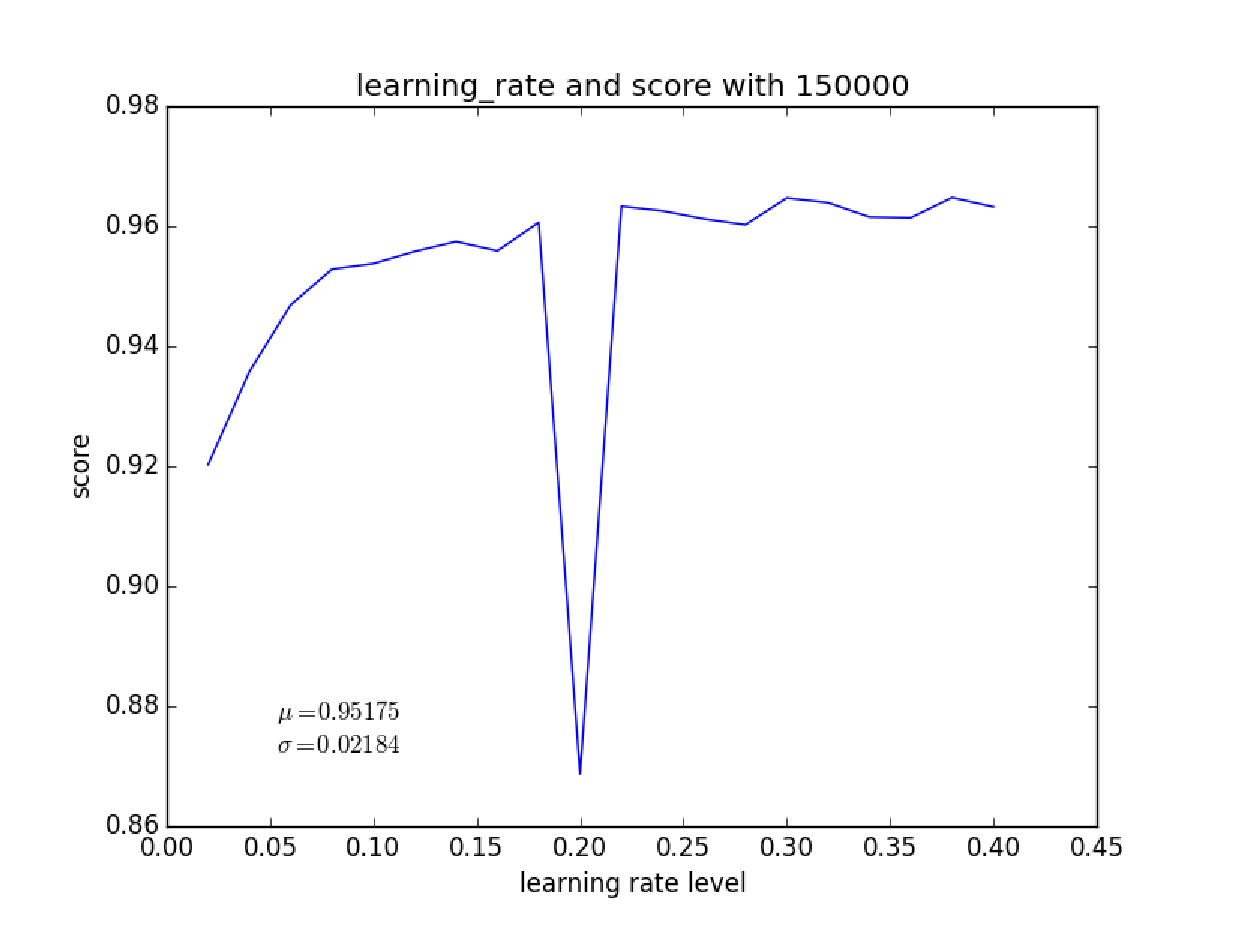
\includegraphics[width=0.45\textwidth]{assets/img/learning_rate_test_mnist.eps}
  \caption{学習率と性能の関係}
  \label{fig:learning-rate-test}
\end{figure}

図\ref{fig:inertia-rate-test}が慣性項の係数を0.0から0.38まで変化させ, 
性能の変化を調べたものである. 
これは学習率を0.3としたときに調べたものであり, 
0.12のとき最も性能が高かった. 
\begin{figure}[htbp]
  \centering
  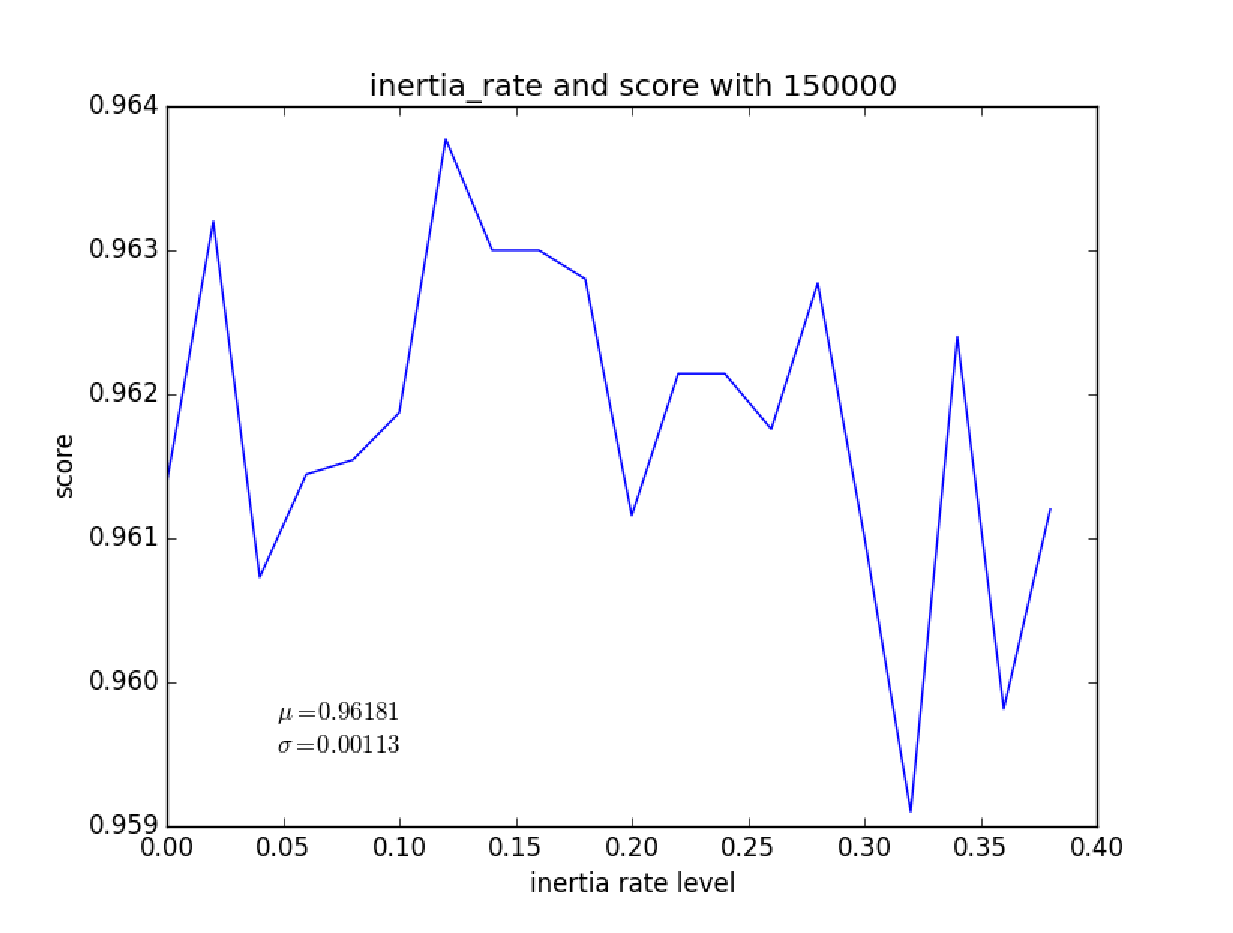
\includegraphics[width=0.45\textwidth]{assets/img/inertia_rate_test_mnist.eps}
  \caption{慣性項の係数と性能の関係}
  \label{fig:inertia-rate-test}
\end{figure}

図\ref{fig:hidden-layer-analyze}は隠れ層のニューロン数を入力層に対する比率
として変化させたときに性能がどう変わるかを調べたものである. 
グラフから, 隠れ層のニューロン数は今回のデータでは0.15あたりが最適で
あるとわかる. 
\begin{figure}[htbp]
  \centering
  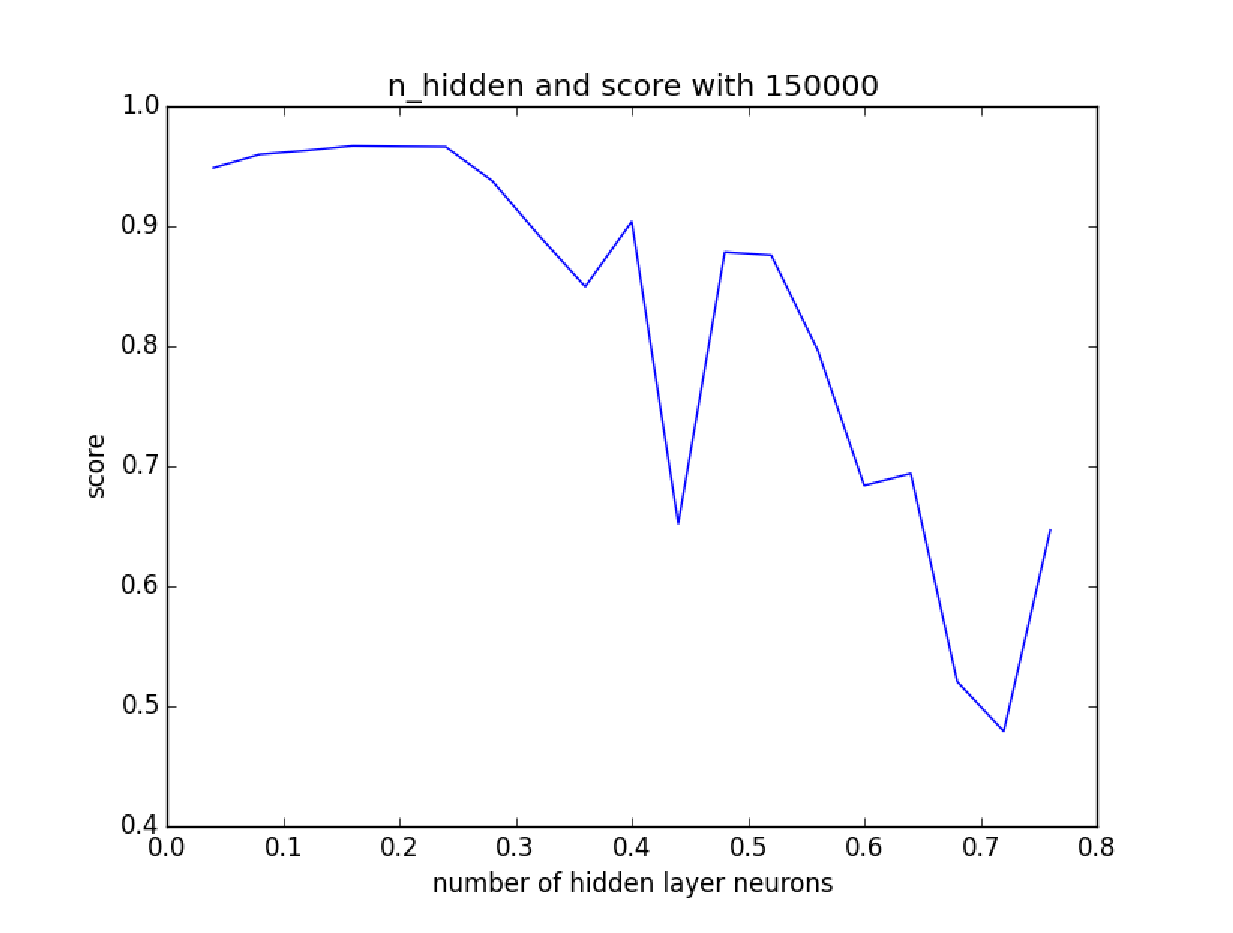
\includegraphics[width=0.45\textwidth]{assets/img/n_hidden_test_mnist_score.eps}
  \caption{隠れ層のニューロン数と性能の関係}
  \label{fig:hidden-layer-analyze}
\end{figure}

図\ref{fig:corruption-level-test}は学習の際のノイズの確率を変化させ, 
それに伴う性能の変化を調べたものである. 
\begin{figure}[htbp]
  \centering
  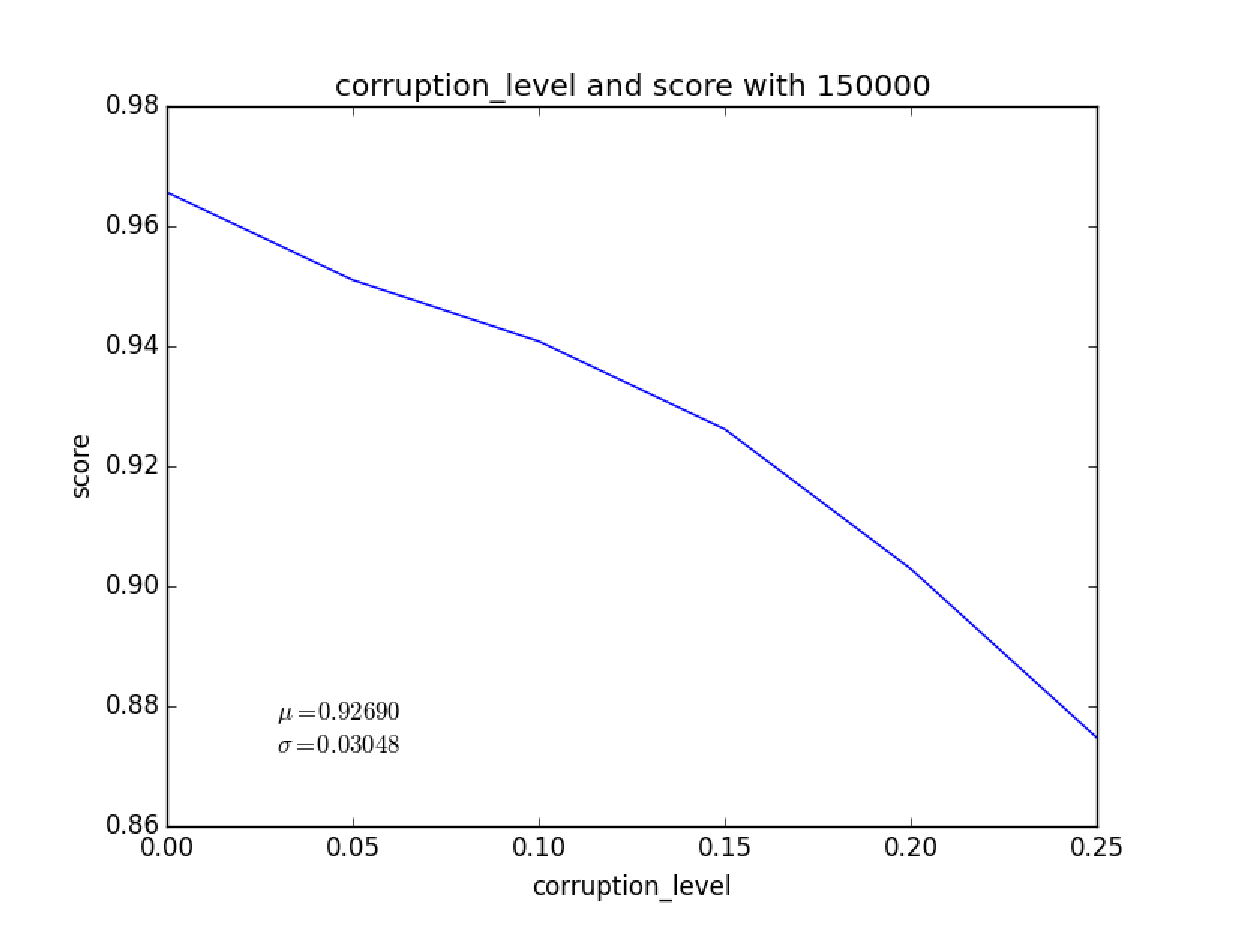
\includegraphics[width=0.45\textwidth]{assets/img/corruption_level_test_mnist.eps}
  \caption{学習の際のノイズと性能の関係}
  \label{fig:corruption-level-test}
\end{figure}

%%%%%%%%%%%%%%%%%%%%%%%%%%%%%%%%%%%%%%%%%%%%%%%%%%%%%%%%

%%%%%%%%%%%%%%%%%%%%%%%%%%%%%%%%%%%%%%%%%%%%%%%%%%%%%%%%
\section{ノイズによる性能変化}
ある確率で画像のピクセル値をランダムな値に変化させるということによって
ノイズをテストデータに発生させ,
予測性能を調べることでノイズの影響を検証した. 

図\ref{fig:noise-0.1}がノイズを10\%,
図\ref{fig:noise-0.25}がノイズを25\%発生させたデータを, 
画像としてプロットしたものである. 

\begin{figure}[htbp]
  \centering
  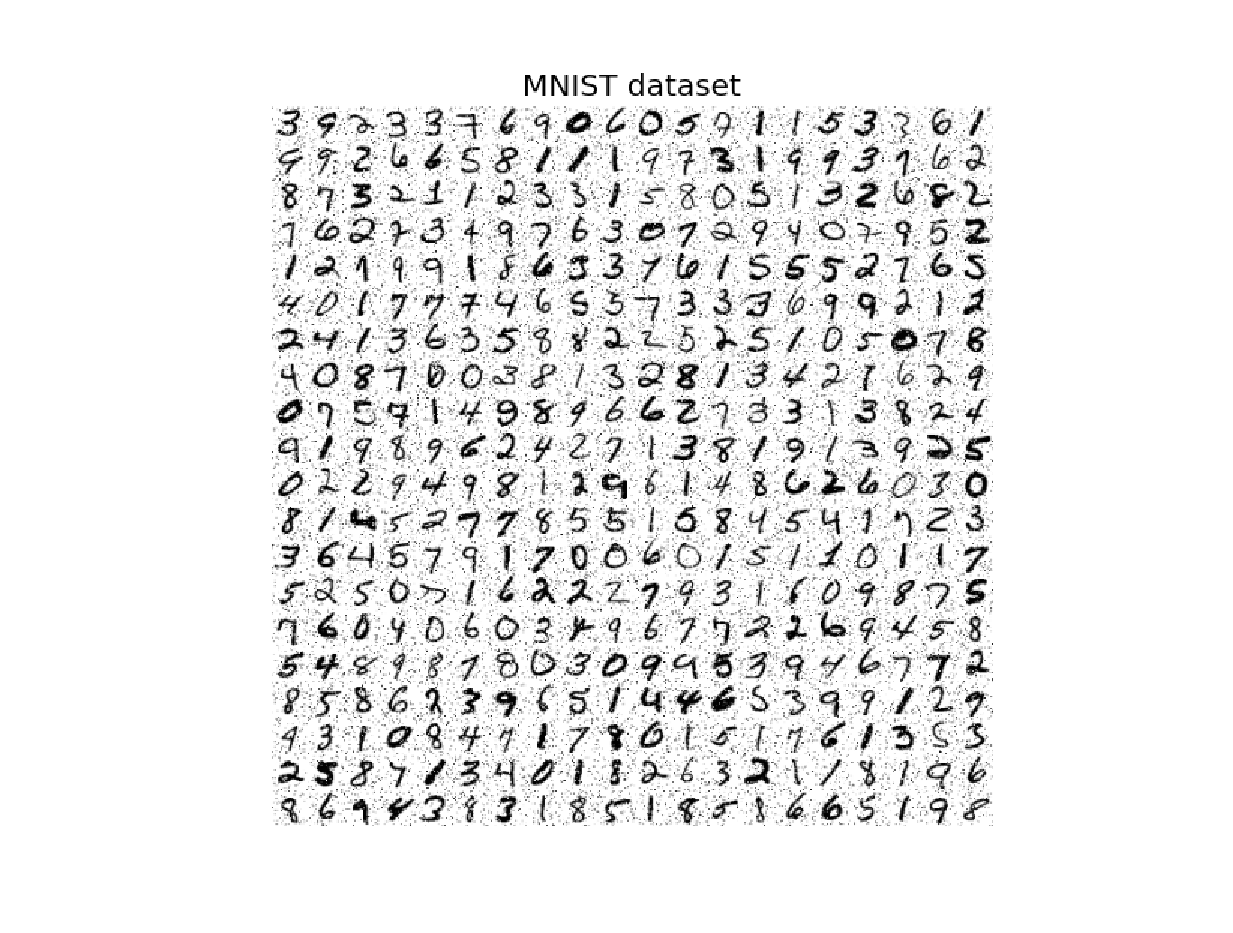
\includegraphics[width=0.45\textwidth]{assets/img/tiled_mnist_nl0.1.eps}
  \caption{ノイズを10\%発生させたデータ}
  \label{fig:noise-0.1}
\end{figure}
\begin{figure}[htbp]
  \centering
  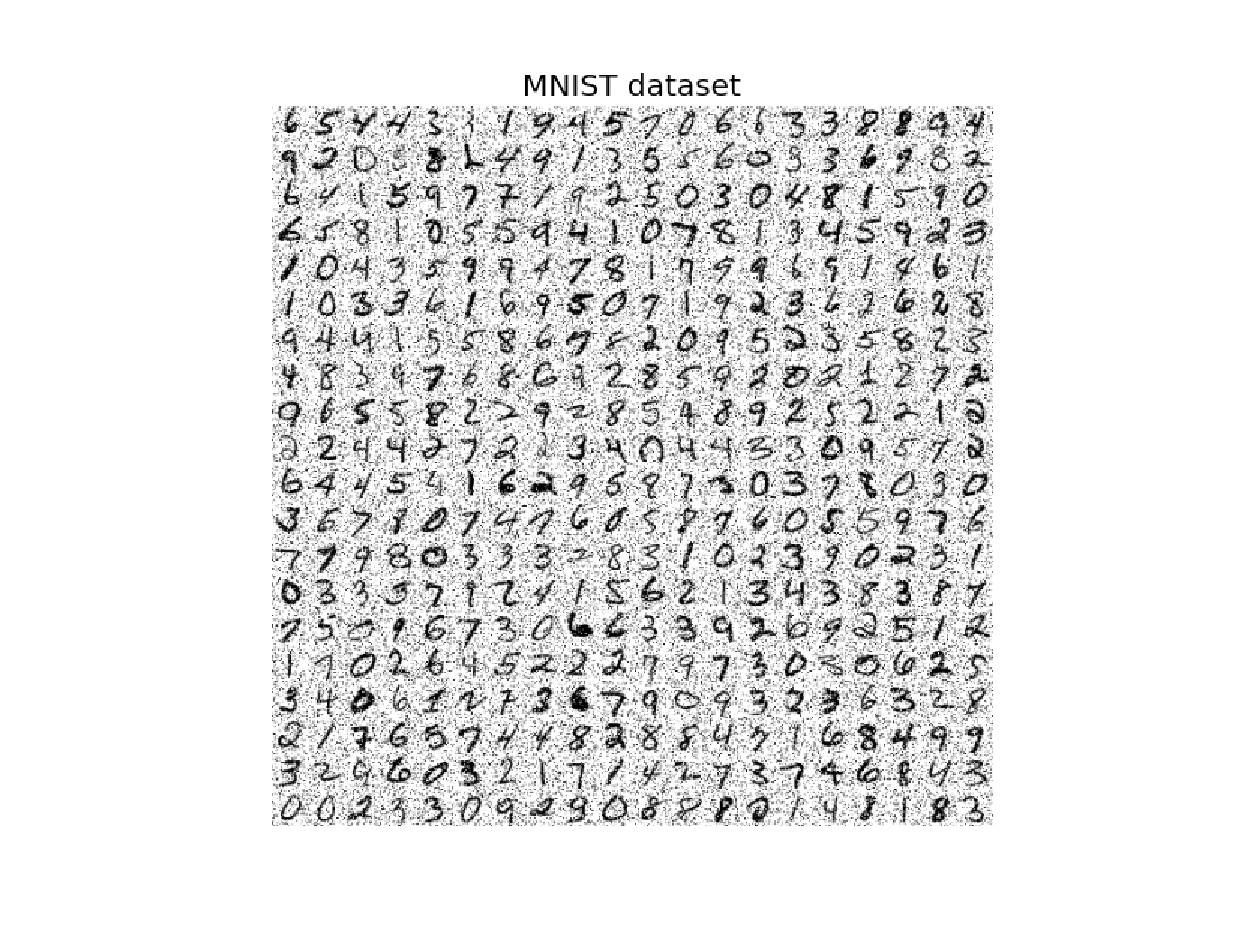
\includegraphics[width=0.45\textwidth]{assets/img/tiled_mnist_nl0.25.eps}
  \caption{ノイズを25\%発生させたデータ}
  \label{fig:noise-0.25}
\end{figure}

\begin{figure}[htbp]
  \centering
  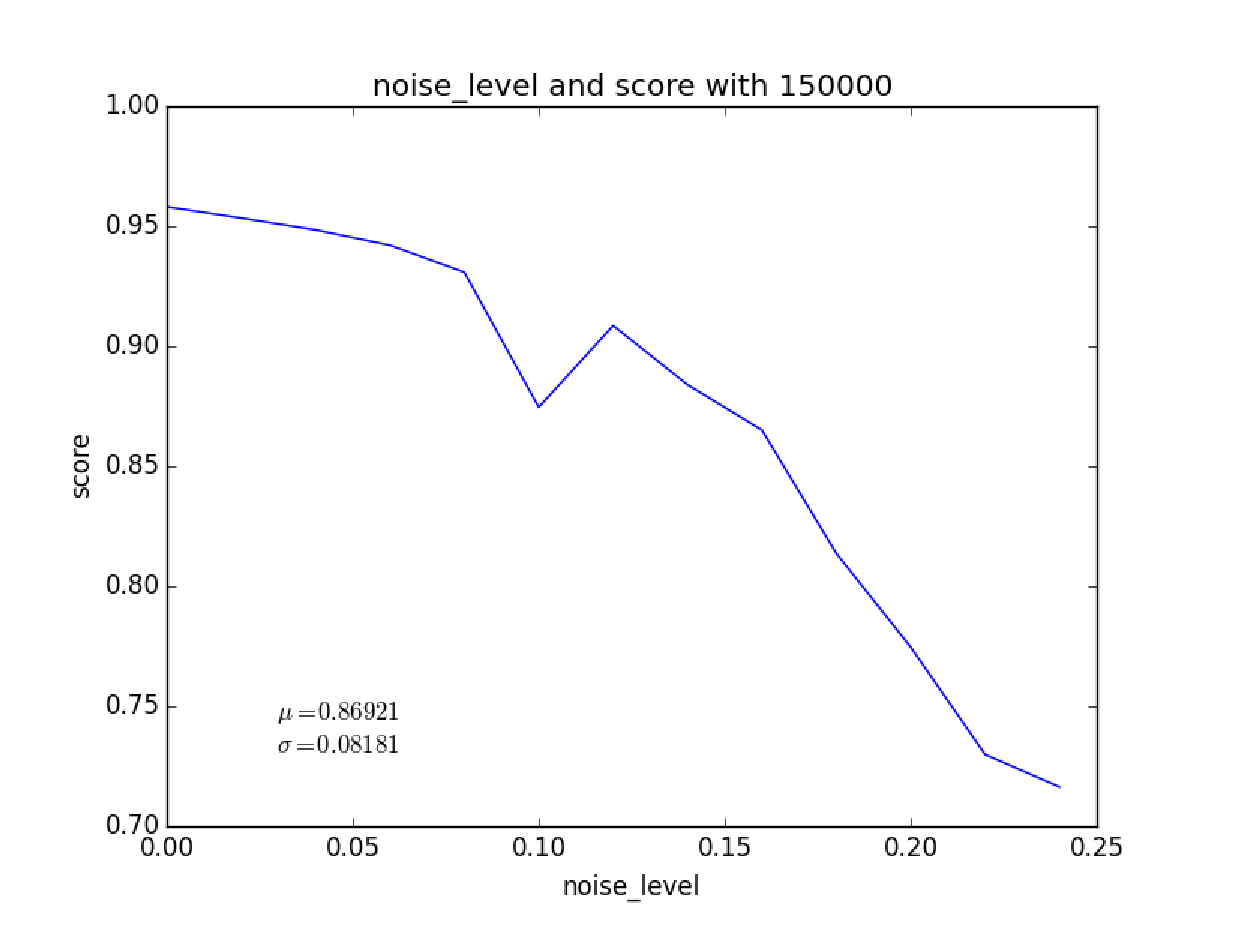
\includegraphics[width=0.45\textwidth]{assets/img/noise_level_test_mnist_cl0.0.eps}
  \caption{ノイズと性能の関係}
  \label{fig:noise-level-test-cl0.0}
\end{figure}

\begin{figure}[htbp]
  \centering
  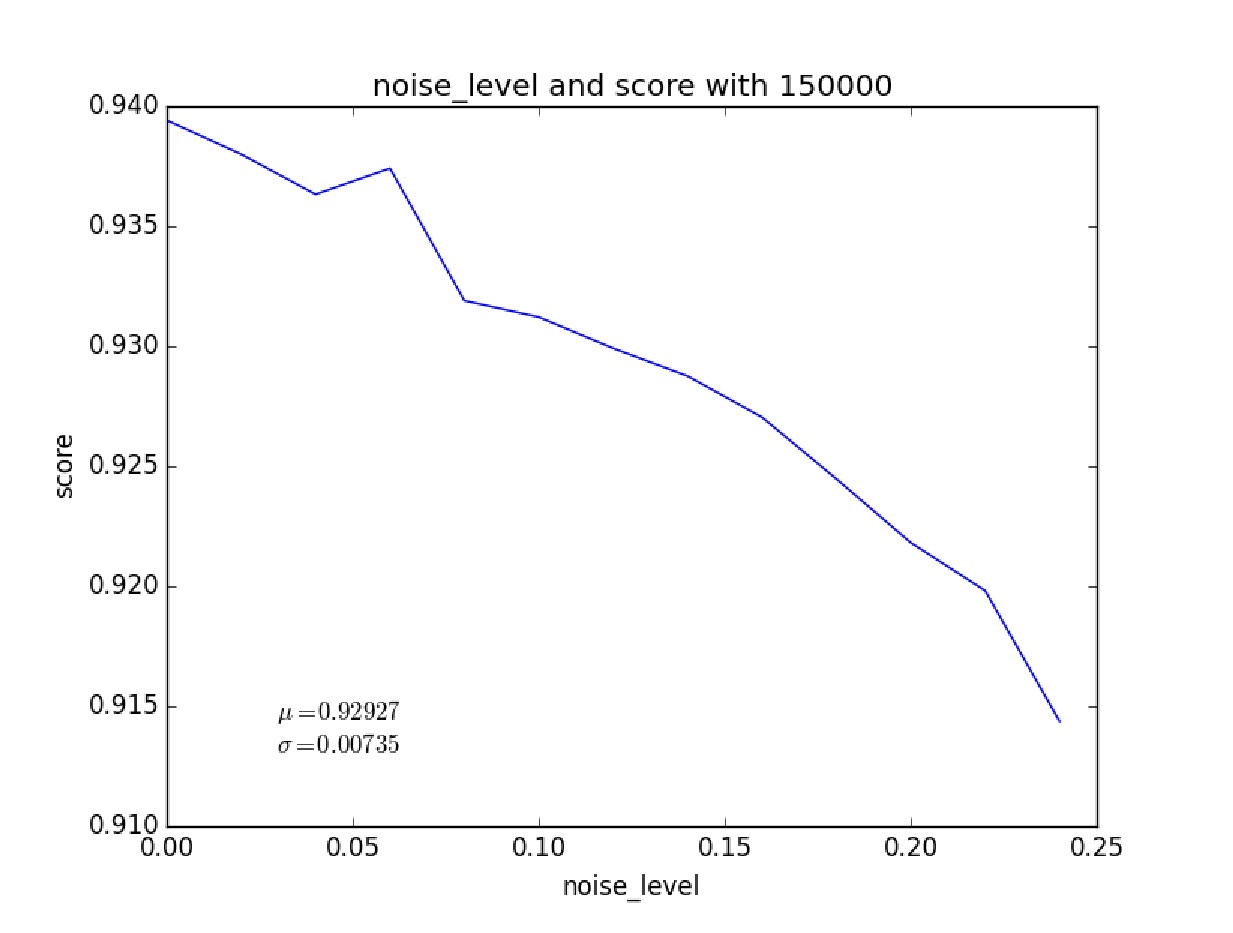
\includegraphics[width=0.45\textwidth]{assets/img/noise_level_test_mnist_cl0.1.eps}
  \caption{ノイズと性能の関係(10\%のノイズを発生させたデータで学習させた場合)}
  \label{fig:noise-level-test-cl0.1}
\end{figure}
%%%%%%%%%%%%%%%%%%%%%%%%%%%%%%%%%%%%%%%%%%%%%%%%%%%%%%%%

%%%%%%%%%%%%%%%%%%%%%%%%%%%%%%%%%%%%%%%%%%%%%%%%%%%%%%%%
\section{中間層のニューロンの役割}
中間層のニューロンの数を変化させ, ニューロン数と識別性能の関係を表した
のが図\ref{fig:hidden-layer-analyze}である. 
このとき, 性能が最も高かった場合と低かった場合についてその重みを
図\ref{fig:hidden-layer-analyze-img-0.16}と
図\ref{fig:hidden-layer-analyze-img-0.72}にプロットした. 

それぞれの図を比較すると, 性能が高かったモデルの重みの方がよりエッジが
はっきりしており, 模様のようなものが見える. 
重みのうち, 値が大きくなっている部分は各入力刺激(入力画像)に対する
受容野のような働きをしており, 結果から, 
その働きが顕著になっている方がより正確な出力を出すことができると言える. 
\begin{figure}[htbp] 
  \centering
  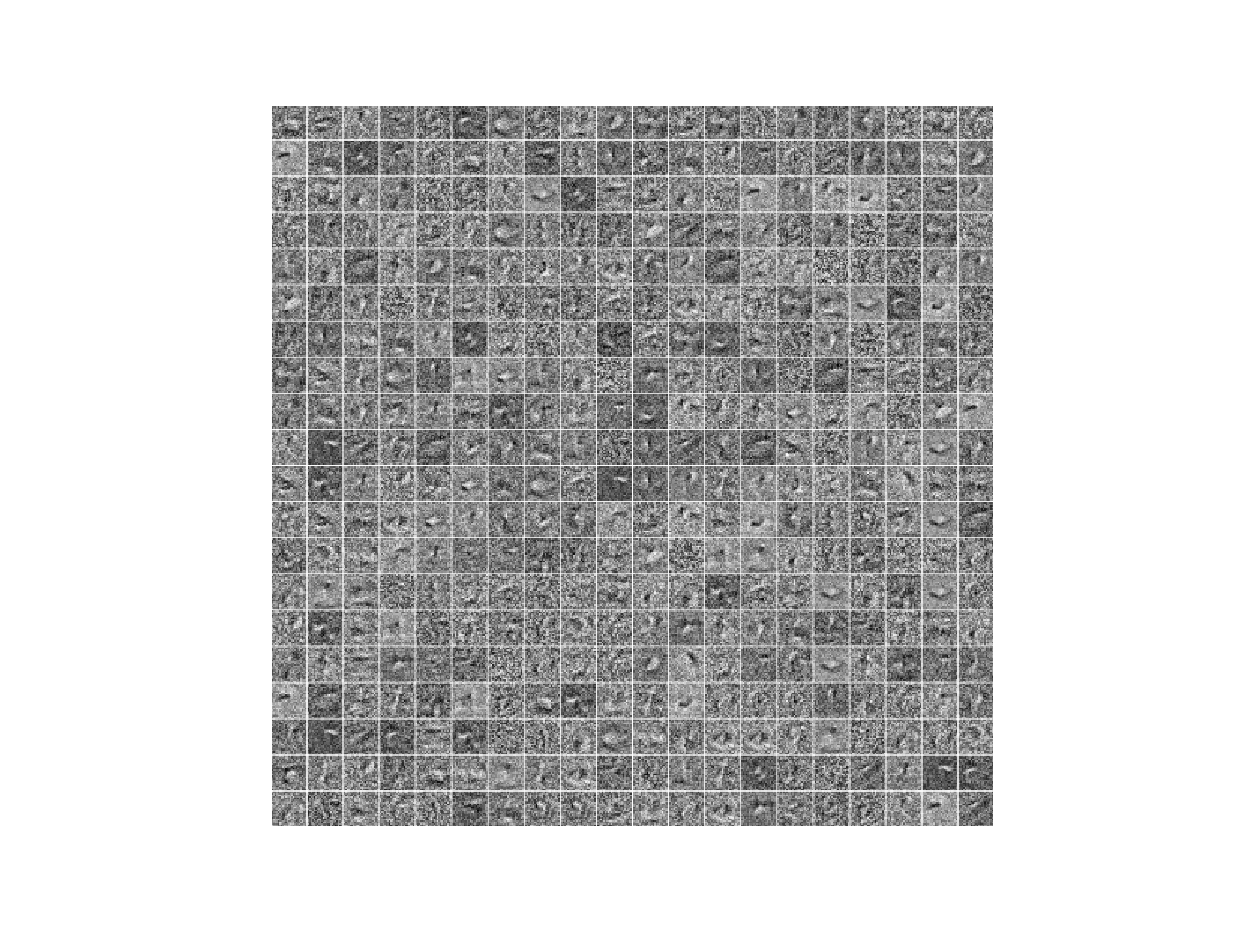
\includegraphics[width=0.45\textwidth]{assets/img/n_hidden_test_mnist_image_nsmpl150000_nh0.16.eps}
  \caption{識別性能が高い場合(中間層0.16)の重み}
  \label{fig:hidden-layer-analyze-img-0.16}
\end{figure}
\begin{figure}[htbp] 
  \centering
  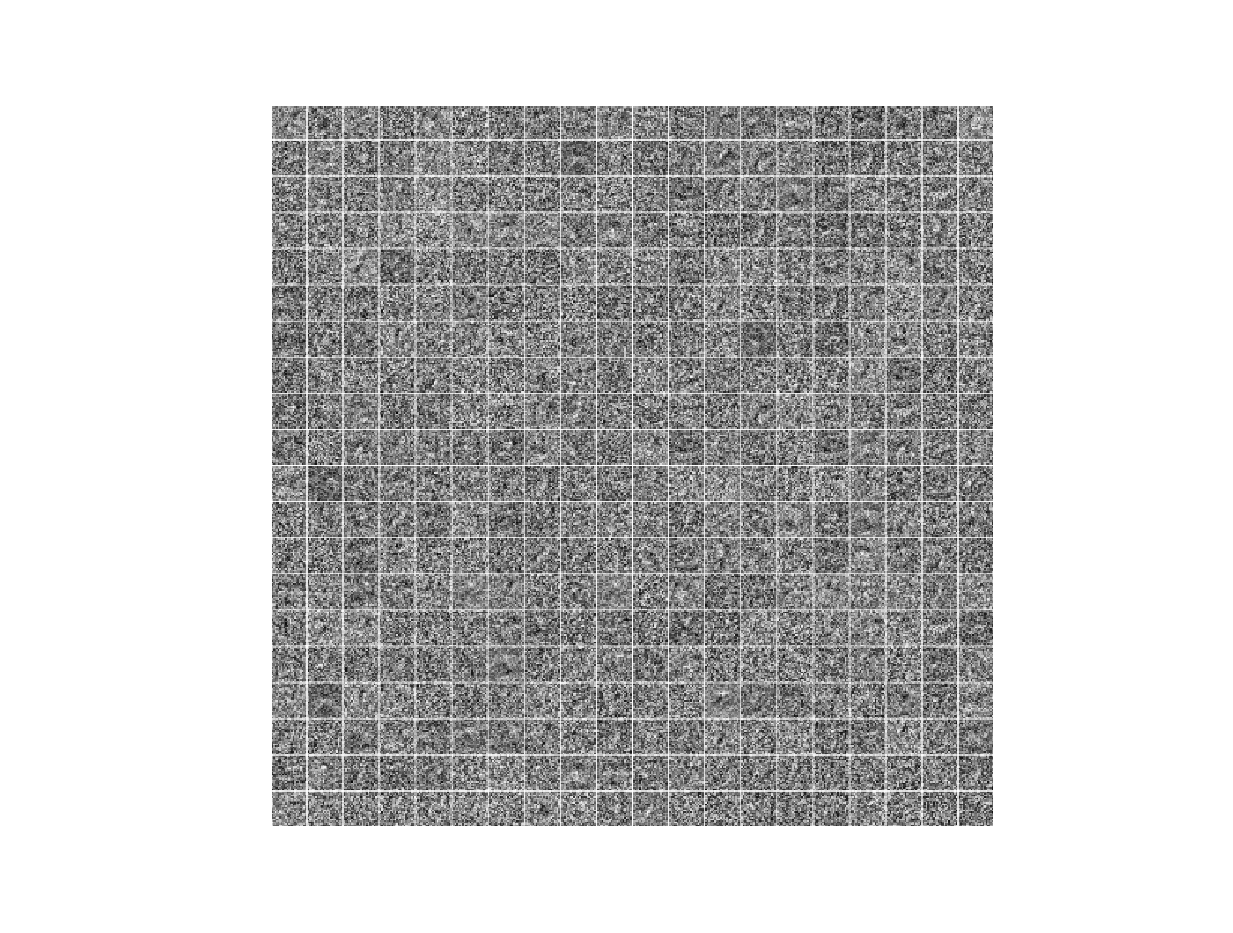
\includegraphics[width=0.45\textwidth]{assets/img/n_hidden_test_mnist_image_nsmpl150000_nh0.72.eps}
  \caption{識別性能が高い場合(中間層0.72)の重み}
  \label{fig:hidden-layer-analyze-img-0.72}
\end{figure}
%%%%%%%%%%%%%%%%%%%%%%%%%%%%%%%%%%%%%%%%%%%%%%%%%%%%%%%%
\section{画像特徴抽出と性能変化}
画像の特徴抽出としてオートエンコーダを用い, その隠れ層の値を入力として, 
性能を調べた. 
精度は0.9474151であった. 
%%%%%%%%%%%%%%%%%%%%%%%%%%%%%%%%%%%%%%%%%%%%%%%%%%%%%%%%
\section{講義の感想}
知的な機械を実現するということを考えさせられる授業で, 現状実現している部分
とその限界, そしてそれを解決するためのアプローチについて丁寧に説明が
あり, 自分で考えながら聞くことができたので力になったと思う. 
必要なところでは黒板を使って説明があるが, 個人的にはもう少し黒板を使った
授業の部分を増やしてほしいと感じた. 


%%%%%%%%%%%%%%%%%%%%%%%%%%
% to insert bibliography %
%%%%%%%%%%%%%%%%%%%%%%%%%%
\begin{thebibliography}{9}
%   \bibitem{inv1} Samuel R.Buss,"Introduction to Inverse Kinematics with Jacobian Transpose,Pseudoinverse and Damped Least Squares methods"
  \bibitem{mnist} Yann LeCun, Corinna Cortes, Christopher J.C. Burges,
    ``MNIST handwritten digit database, Yann LeCun, Corinna Cortes and Chris Burges'',
    http://yann.lecun.com/exdb/mnist/
\end{thebibliography}

%%%%%%%%%%%%%%%%
% end document %
%%%%%%%%%%%%%%%%
\end{document}